\chapter{Instrument Overview}
\label{ch:instruments}

We are in the age of precision cosmology, and measurements of the CMB spectra continue to improve in sensitivity.  Now, to measure the CMB polarization anisotropies, scientists are pushing forward the sensitivity of the instruments by increasing detector numbers, improving detector sensitivity, and controlling optical systematics, to name a few.  For example, the Atacama Cosmology Telescope (ACT), a ground-based cosmology experiment, used roughly 3000 bolometric detectors.  The Simons Observatory is scaling its detector count up to more than 50,000 bolometric detectors in order to improve mapping speed and sensitivity.  Looking ahead, the CMB-S4 collaboration, the next-generation cosmology project, plans to scale up even further: to roughly 500,000 detectors.  This, along with the many other improvements in instrumentation, aim to detect the smallest signals of the CMB polarization spectra.

In this chapter, I describe two ground-based cosmology experiments covered in this work: the Atacama Cosmology Telescope (ACT), an operational cosmology experiment~\cite{act_inst}, and the Simons Observatory (SO), the next-generation cosmology experiment~\cite{so19}. 

\section{Atacama Cosmology Telescope}
\begin{figure}[ht]
    \centering
    \includegraphics[width=\textwidth]{Figures/Site_Drone_Picture_July_2019.jpeg}
    \caption{The Simons Observatory (SO) and Atacama Cosmology (ACT) site in the Atacama Desert, Chile. The ACT telescope sits within a ground-shield which can be sen in the bottom center.  The outer ground screen protects the telescope from stray light.  The inner co-moving ground-screen further protects the telescope from stray light during observations.}
    \label{fig:act_so_site}
\end{figure}

The full ACT is shown in Figure~\ref{fig:act_site}.  Figure~\ref{fig:act_inst} shows the ray-trace of ACT's off-axis Gregorian geometry with two reflectors which guide photons into the receiver cabin.  Within the receiver cabin, three optics tubes re-simage the Gregorian focus onto the detector arrays~\cite{thornton_2016}.

\begin{figure}
    \centering
    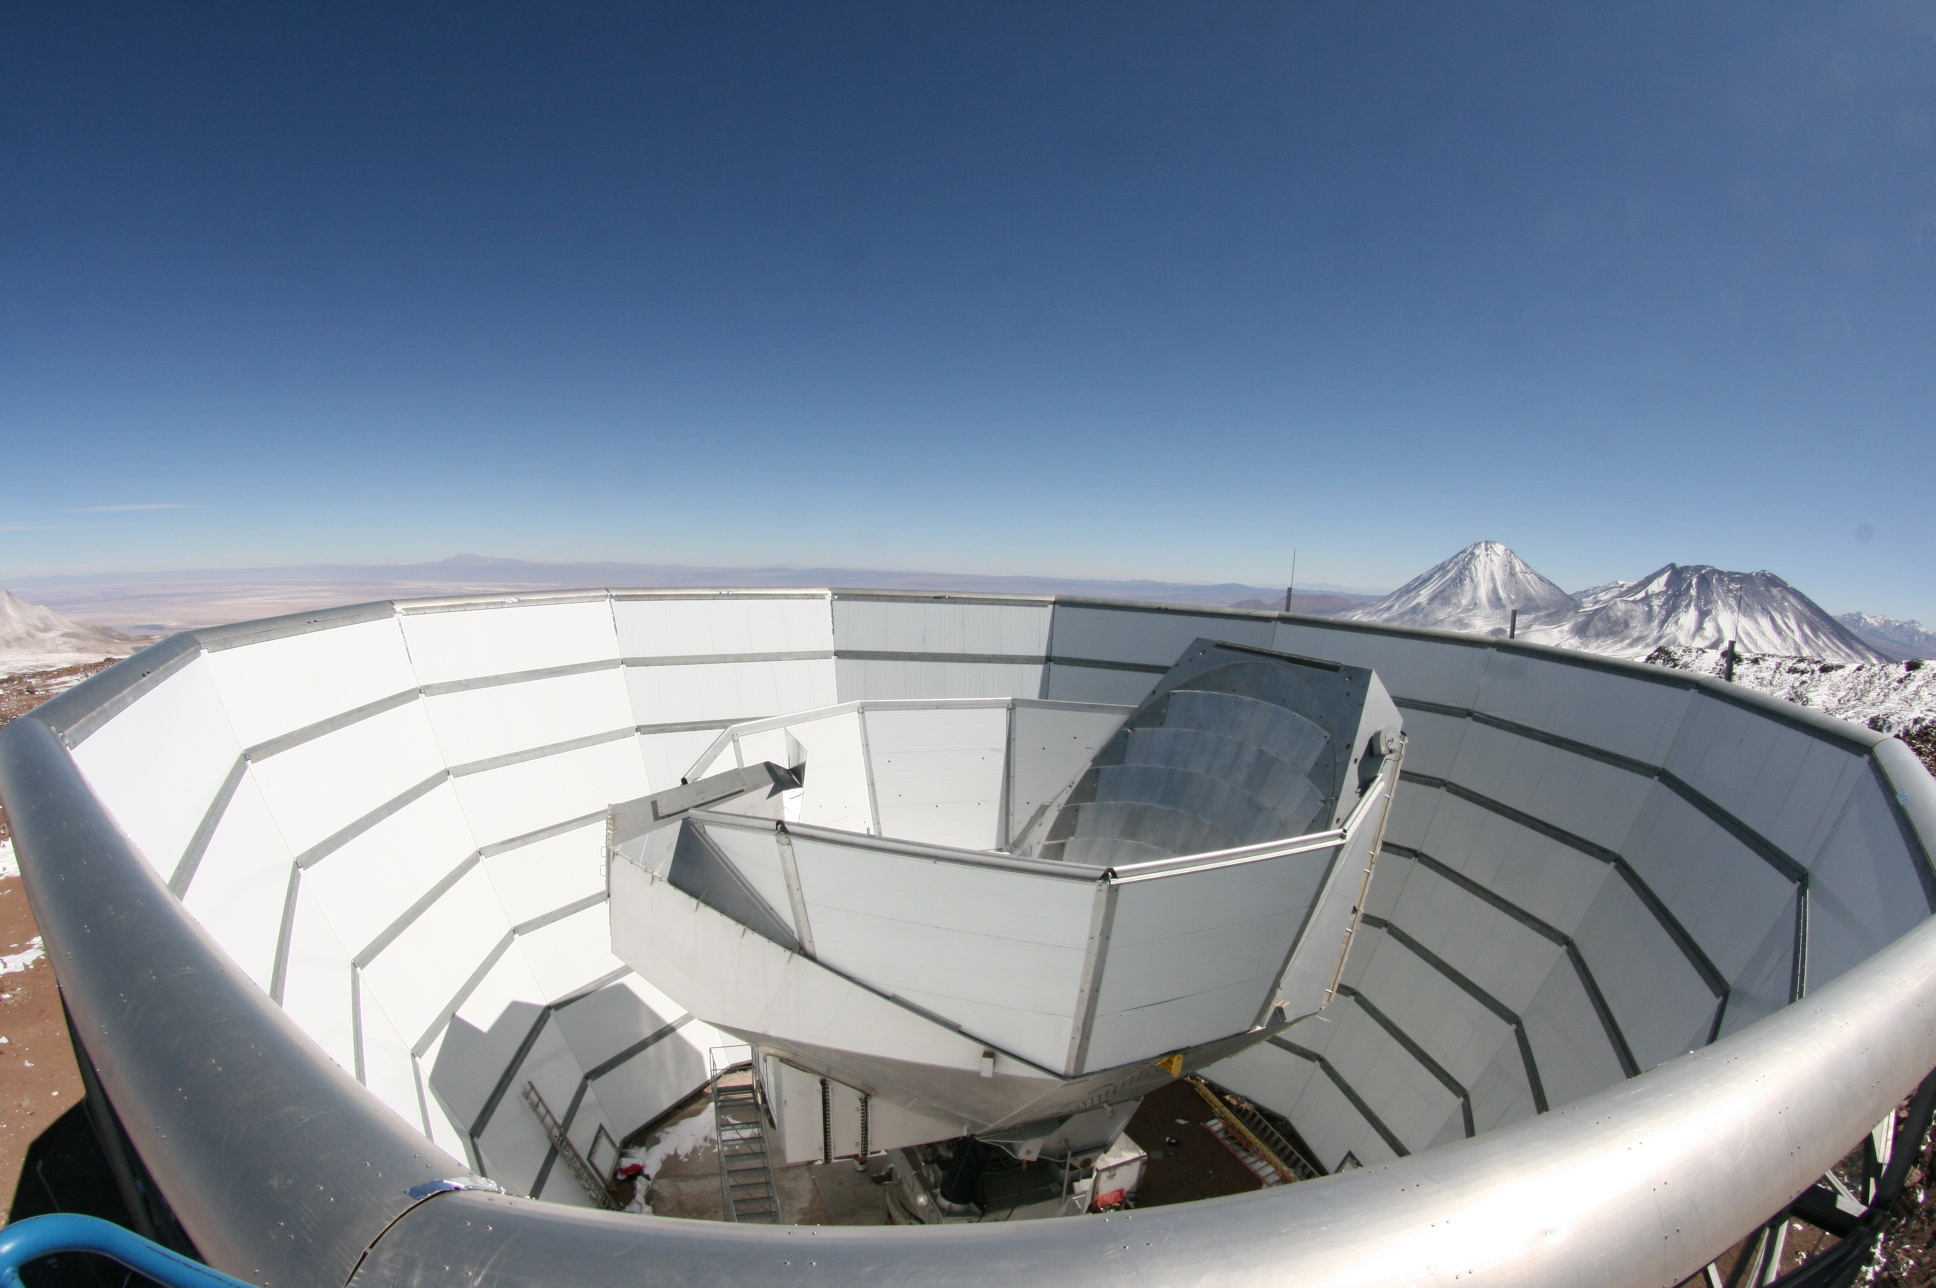
\includegraphics[width = .7\textwidth]{Figures/act_inst_close.jpeg}
    \caption{The Atacama Cosmology Telescope, surrounded by its outer ground screen. The inner co-moving screen further shields the instrument from any stray-light.  One can see the top of the primary mirror behind the co-moving screen.}
    \label{fig:act_site}
\end{figure}

\begin{figure}[t]
    \centering
    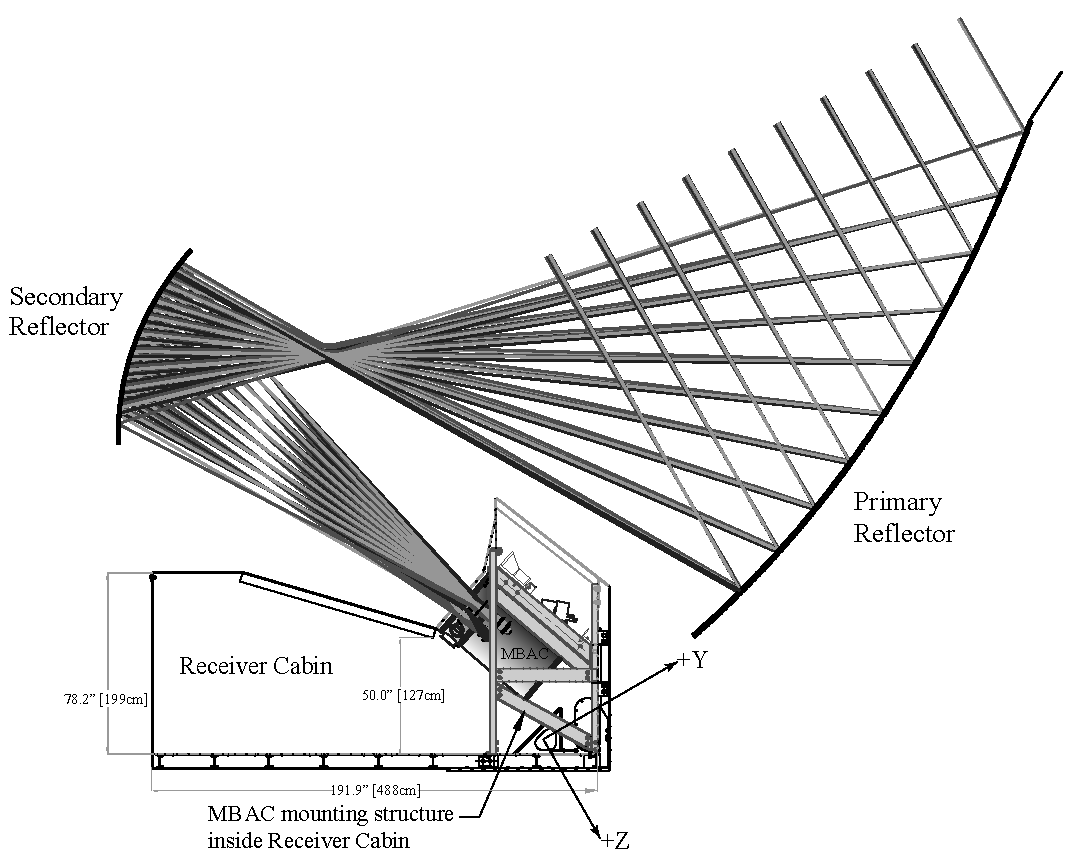
\includegraphics[width = .8\textwidth]{Figures/act_inst.pdf}
    \caption{Ray-trace diagram of the Atacama Cosmology Telescope~\cite{act_inst}.  The telescope is an off-axis Gregorian with two reflectors: the primary is 6\,m in diameter and the secondary 2\,m.  The rays trace into the Millimeter Bolometer Array Camera (MBAC) cryostat which houses the telescope's detectors.}
    \label{fig:act_inst}
\end{figure}

In Chapter~\ref{ch:actbeams} I present the characterization of the ACT beam using point-source stacking.  From the stacking, I also determine polarization leakage in the maps.

\begin{table}[t]
    \centering
    \begin{tabular}{|l|l|l|l|} \hline
        \textbf{ Parameter} &  \textbf{PA4 F150} &  \textbf{PA5 F090}  &  \textbf{PA6 F090}  \\ \hline \hline
        Number of Bolometers & 510 & 510 & 510\\\hline
        Center Frequency (GHz) & 150\,GHz & 90\,GHz & 90\,GHz\\\hline
        Base Temperature & 100\,mK & 100\,mK & 100\,mK\\\hline
        % Angular Resolution & 1 arcmin &1 arcmin &1 arcmin\\\hline
        % Solid Angle & & &\\\hline
        % Sky Coverage & & &\\\hline
    \end{tabular} \caption{ACT Key Characteristics.}
    \label{tab:act}
\end{table}

\section{The Simons Observatory}

SO will test cosmic inflation during the early universe, characterize the primordial perturbations, measure the effective number of relativistic species and the sum of the neutrino masses, and improve our understanding of galaxy evolution and the era of cosmic reionization~\citep{so19,so_science}. 

An ongoing challenge in cosmology instrumentation has been characterizing the polarization spectra of the CMB.  Specifically, the B-mode polarization of the CMB offers a unique window into early-universe physics~\cite{}.  Because scalar perturbations generate E-mode polarization, a measurement of the B-mode polarization directly quantifies the scalar-to-tensor ratio $r$.

The CMB serves as a backlight for large-scale structure, therefore providing insights into gravitational lensing, and ...

The resolution of SO will result in a catalog of extragalactic sources, including active galactic nuclei (AGN), dusty star-forming galaxies, and transient sources including Gamma Ray Burst (GRB) afterglows~\cite{so_science}.  SO expects to catalog 10,000-15,000 AGN sources at flux-densities above 7\,mJy~\cite{Tucci_2011}.  The low frequency coverage of SO will compliment comparison work with other catalogs (e.g. VLA/VLASS, ASKAP/EMU, MeerKAT/MIGHTEE)~\cite{so_science}.  Dusty star-forming galaxies seen by SO will include local galaxies ($z<0.1)$ and high redshift galaxies (approximately $2<z<4$), and strong lensed galaxies beyond this range~\cite{Marrone_2017}.

\begin{figure}[t]
    \centering
    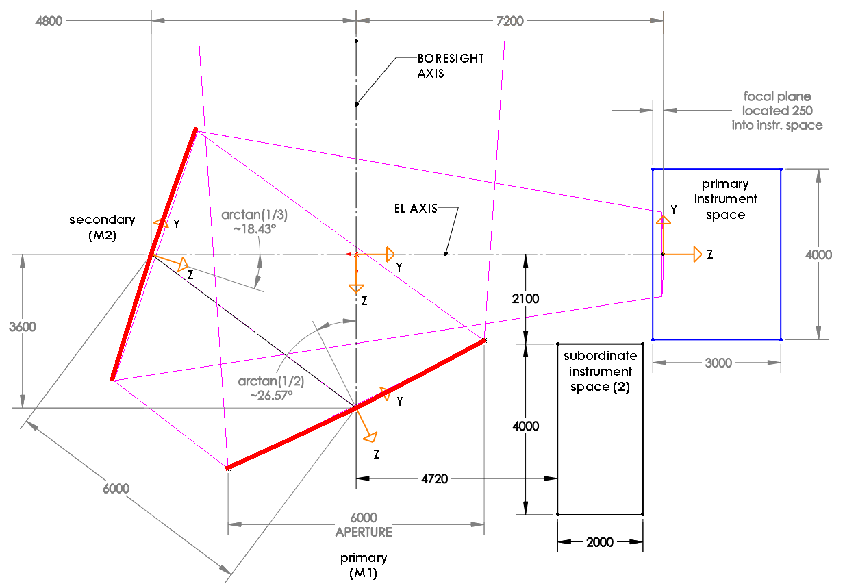
\includegraphics[width = .9\textwidth]{Figures/LAT_rt.pdf}
    \caption{Ray-trace diagram of the Simons Observatory Large Aperture Telescope~\cite{Parshley_2018}.  The telescope is a cross-Dragone with two reflectors, both 6\,m in diameter.  The rays trace into the Large Aperture Telescope Receiver (LATR) cryostat which houses 13 optics tubes.  The optics tubes guide the photons onto the detectors in the focal plane, which are cooled to 100\,mK.}
    \label{fig:so_inst}
\end{figure}

The Simons Observatory (SO) is a series of millimeter-wave telescopes designed to observe the Cosmic Microwave Background (CMB) temperature and polarization signals to an unprecedented sensitivity~\cite{gali18, so19}. With the combination of one Large Aperture Telescope (LAT)~\cite{xu/etal:2020c, zhu18, orlo18, coppi/etal:2018} and three Small Aperture Telescopes (SAT)~\cite{ali20}, the experiment will measure the temperature and polarization anisotropy of the cosmic microwave background with $\sim$\,70,000 background noise limited detectors operating at $\sim$\,100\,mK. 

The Simons Observatory was deployed in the Parque Astronomico located in the Atacama Desert in Chile. The telescope site is situated at an elevation of 5200 meters near the peak of Cerro Toco at $22 ^\circ$ 57' S, $67^\circ$47' W. The arid conditions and elevation at the site minimize contamination to millimeter wave signals from water vapor. 

\begin{table}[ht]
    \centering
    \begin{tabular}{|l|l|l|l|} \hline
        \textbf{ Parameter} &  \textbf{LF} &  \textbf{MF}  &  \textbf{UHF}  \\ \hline \hline
        Number of Bolometers & $>$20,000& $>$20,000& $>$20,000\\\hline
        Base Temperature & 100\,mK & 100\,mK & 100\,mK\\\hline
        Angular Resolution & 1 arcmin &1 arcmin &1 arcmin\\\hline
        Solid Angle & & &\\\hline
        Center Frequency (GHz) & 27-270\,GHz & 27-270\,GHz & 27-270\,GHz\\\hline
    \end{tabular} \caption{SO Key Characteristics.}
    \label{tab:so}
\end{table}

\subsection{Large Aperture Telescope}

The primary mirror is 6\,m in diameter and constructed out of 77 individual adjustable panels, while the secondary mirror is 6\,m in diameter and constructed out of 69 adjustable panels \cite{gali18}.

Figure~\ref{fig:LATR_Cross} shows a cross-section of the LAT Receiver, which houses up to thirteen optics tubes~\cite{Xu_2021}.

Chapter~\ref{ch:ot_holo} presents radio holography measurements of the LAT optics tube, where I characterize the optical performance of the LAT Receiver optics tube.

\subsection{Small Aperture Telescope}

The Small Aperture Telescope (SAT) optical design is a 0.42\,m diameter refractive telescope.  Three SATs will measure the largest angular scales visible from the Atacama Desert.

In Chapter~\ref{ch:sat_holo}, I present radio holography measurements of the SAT optics tube.